\subsection{The Raw Data tab}
\label{sec:raw_data_tab}

This tab allows to specify and inspect the input data, to specify how deep into the reduction cascade to go
(reduction target), to configure the association preference, and, finally, to create the dataset to reduce.

There are 5 main buttons:
\begin{itemize}
\item {\bf Select the input data}. The button "Select Inputs" opens a window that allows to specify the
  directory where the input data are located (Figure \ref{fig:select-inputs-dialog}). 

\begin{figure}[h!]
\centering
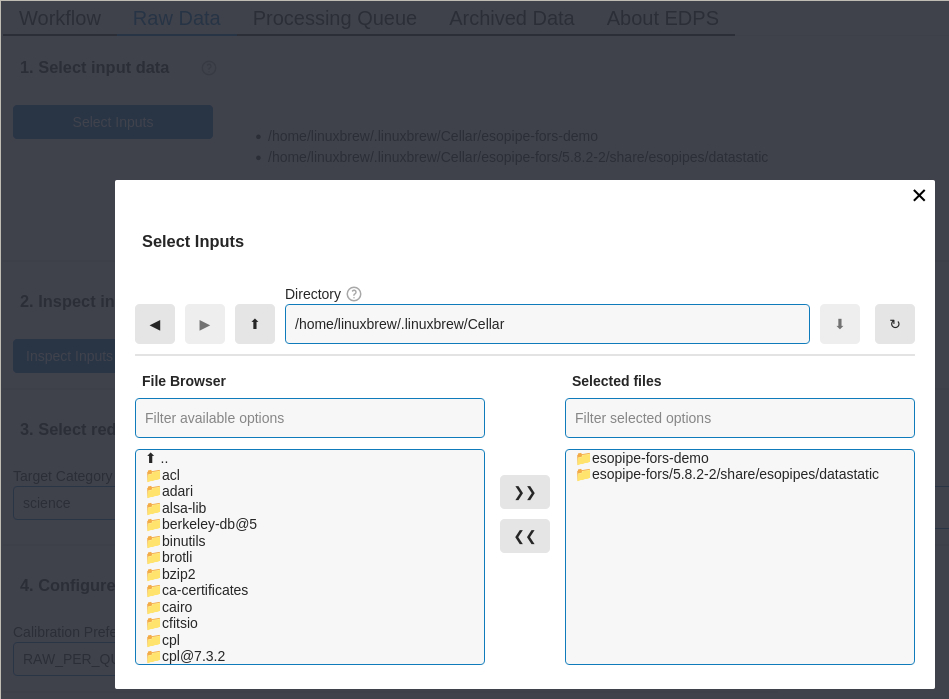
\includegraphics[width=0.9\textwidth]{figures/select-inputs-dialog.jpg}
\caption{The Select Inputs dialogue box.}
\label{fig:select-inputs-dialog}
\end{figure}


\item {\bf Inspect the input data}. 
\label{list:inspect}
The button "Inspect Inputs" allows to inspect the input files. Press this button and a table with the the
  list of input files appears.
  The first part of the table (Figure \ref{fig:inspect_1}) shows the list of the input files, grouped by category. Click on the arrow of each
  category to show the files
  within. Buttons on the left side of each file allows to visualize it
  either with {\tt fv} or `{\tt ds9} (if present in your system).
  The second part of the table (Figure \ref{fig:inspect_2}) allows to inspect the headers of the various extensions, and also
  it allows to inspect the data extension with interactive Python tools.


\begin{figure}[h!]
\centering
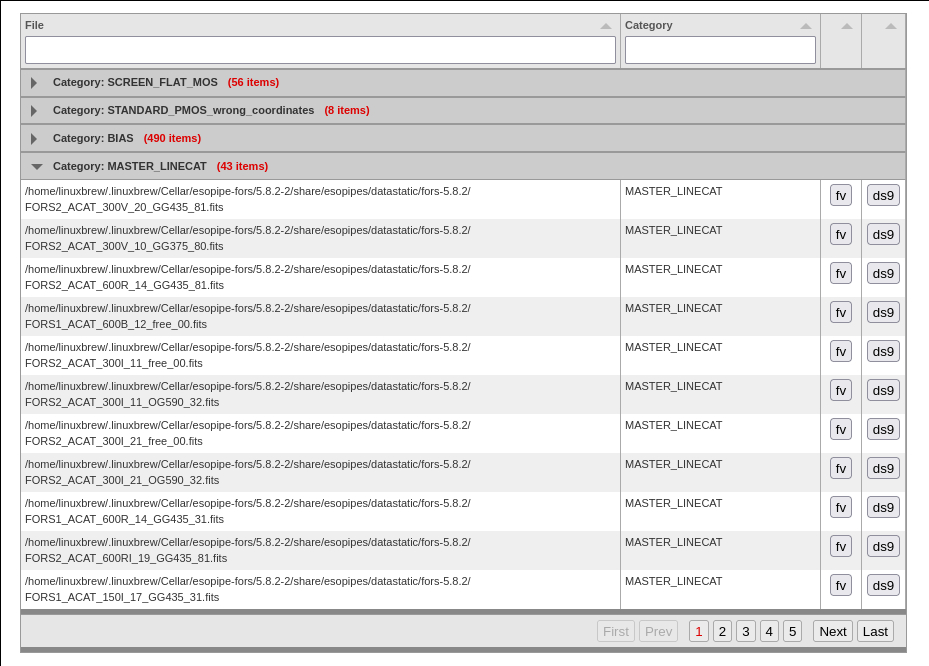
\includegraphics[width=0.9\textwidth]{figures/inspect_1.jpg}
\caption{The Inspect Inputs dialogue box: list of categories.}
\label{fig:inspect_1}
\end{figure}

\begin{figure}[h!]
\centering
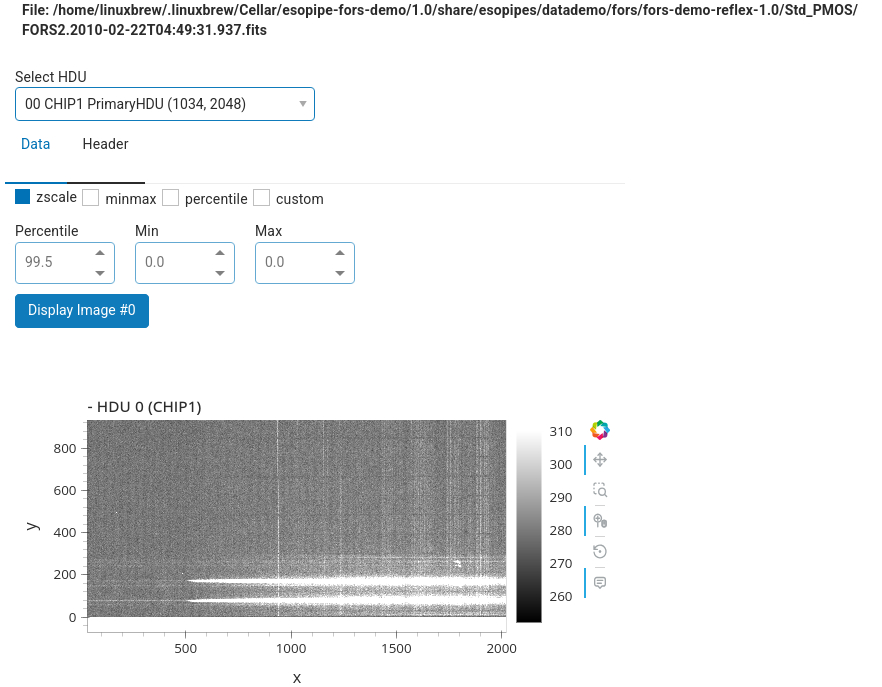
\includegraphics[width=0.9\textwidth]{figures/inspect_2.jpg}
\caption{The Inspect Inputs dialogue box, inspection of extensions.}
\label{fig:inspect_2}
\end{figure}


\item {\bf Select reduction target}. This window (Figure \ref{fig:select_reduction_target}) allows to specify the final steps of the reduction cascade, the so-called
  "target tasks".
  The tasks, i.e. the various steps of the reduction flow, are grouped by categories, which can be selected from the
  drop-down menu "Target Category".

  \edps\ processes all the data until the specified target tasks, and triggers all the tasks down in the reduction cascade
  that are needed
  to trigger the target task. For example, if the target task is "science", and the reduction cascade foresees that also
  the "bias" and "flat\_field" tasks are needed to provide the necessary calibrations, then EDPS will process
  all and only the biases and the flat fields that are needed to reduce the science data. If there are other biases or
  flat fields that are
  not needed for the specified science exposure, they are not reduced. On the other hand, if the specified target task
  is
  "flat\_field", then EDPS will reduce all the flat field exposures, plus all and only the biases that are needed for
  those flat fields.

\begin{figure}[h!]
\centering
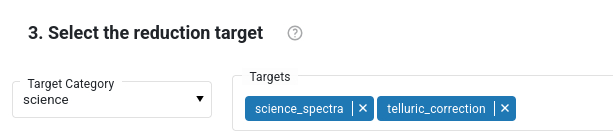
\includegraphics[width=0.9\textwidth]{figures/select_reduction_target.jpg}
\caption{The Select Reduction Target box.}
\label{fig:select_reduction_target}
\end{figure}


  Individual tasks within that category are listed in the "Targets" bar. In Fig. \ref{fig:select_reduction_target},
  the "Science" category is shown, that contains the tasks called science\_spectra and telluric\_correction. The
  categories and the tasks depends on the loaded workflow. The category "science" is specified by default.
  The category "all" shows all the tasks in that workflow. Tasks that are not desired, can be removed from the list.
  The category "qc1calib" triggers all the calibration and instrument monitoring tasks, but it does not process
  scientific images.
  Other target categories are specific for Paranal operations, and are not needed for the general user.


\item {\bf Select the workflow parameters}
  This windows allows to specify the so called "workflow parameters", e.g. parameters that define the strategy
of the reduction or, as in case of FORS (see Figure \ref{fig:select_workflow_parameters}), the criteria on how to group files to combine.
Workflow parameters can influence which files enter a dataset. Click on the parameter name to visualize a short description.
Every workflow has a different list of workflow parameters. 

  There are several "Parameter sets" that can be selected, e.g. sets whose parameter values are predefined according to specific
use cases. By default, the "science" parameter set is loaded, which contains the settings for the most science use cases. 
This is the recommended parameter set to use or, eventually modify.
Other parameters sets are qc0\_parameters (for quick inspection at Paranal), idp\_parameters (the set used by ESO to 
populate the science archive), default\_parameters (to automatically process calibrations in Chile). Other workflows
might contain additional parameters sets, depending on the use case.
Note that the parameters shown in this window are only the workflow parameters, e.g. those that can determine the 
content of the dataset. Other parameters (e.g. recipe parameters) can be configured in the Reduction Queue individually for each dataset (Section \ref{configuration_editor}).




\begin{figure}[h!]
\centering
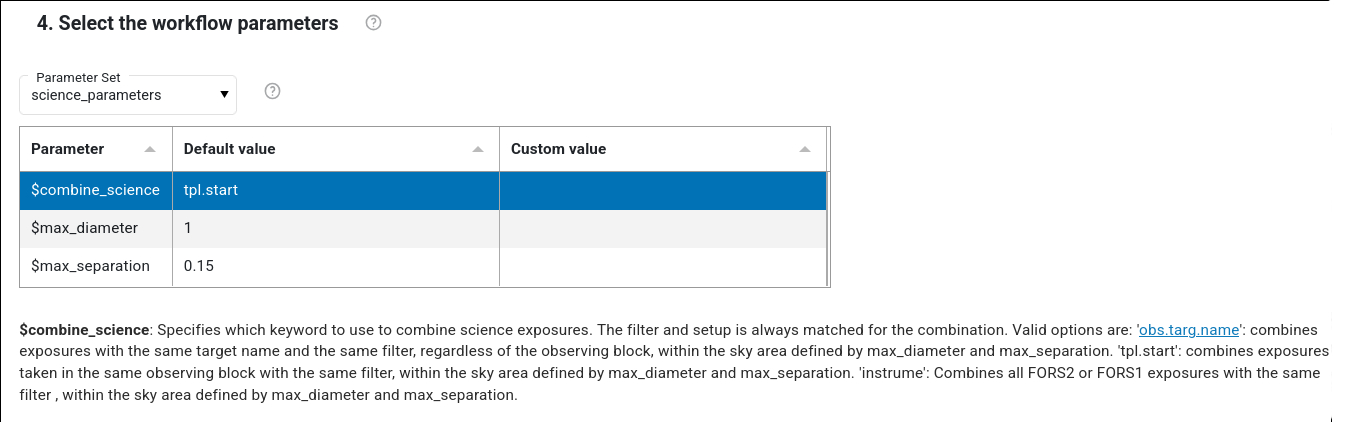
\includegraphics[width=0.9\textwidth]{figures/select_workflow_parameters.jpg}
\caption{The Select Workflow parameters window. Click on a parameter to display the description.}
\label{fig:select_workflow_parameters}
\end{figure}

\label{list:create_datasets}

\item {\bf Create Dataset}. 
This steps creates the datasets to be reduced until the specified reduction target.
 
  The menu "Calibration preference" allows to specify the preferences in associating calibrations (e.g., raw or  master calibrations). The various preferences are described in Section \ref{list:association_preferences}.
  
  For regular science reduction the options raw\_per\_quality\_level (default) or master\_per\_quality\_level are recommended.

  Press the "Create Dataset" blue button to create the datasets. 
  Datasets, together with all the calibrations needed to process them, are listed in a table.  Selected datasets can be sent to the processing queue by pressing  the "Submit to Reduction Queue" blue button. 

  {\bf Important notes:}
  \begin{itemize}
  \item When submitting a dataset, the reduction 'does not start automatically'. To process a dataset, please, go the the Reduction Queue tab.
 \item You cannot submit to the Reduction queue datasets that are already submitted. 
 \item If datasets are already generated, the "Create dataset" button is not active. Because a dataset is defined by the reduction 
    target and the files it contains, to generate new datasets, one has either to specify new input files, change workflow 
    parameters that change the way files are included (e.g., different combination strategy) or change the association preference. 
    \end{itemize}

\begin{figure}[!ht]
\centering
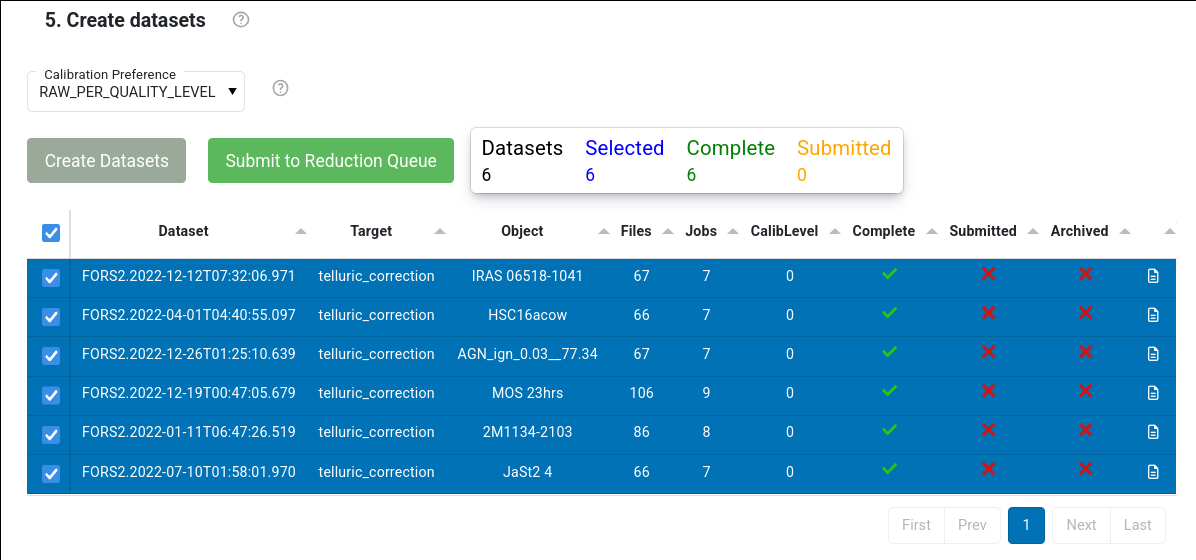
\includegraphics[width=0.9\textwidth]{figures/create-dataset.jpg}
\caption{The Create Dataset section. The table shows the available datasets, with some information on the content, and allows to mark datasets for reduction.}
\label{fig:create-dataset}
\end{figure}

  
  The table shows information about the number of jobs, of files, if a dataset is complete, if it has been submitted to the reduction queue, 
  of whether the final products have been archived.
  It also indicates the {\bf CalibLevel}, i.e. a number indicating the quality of the associations for that datasets. If CalibLevel is 0, it means that 
  all the associations are within a "safe" time interval foreseen by the calibration plan of that instruments. 
  Higher numbers indicate associations of lower quality. More information on the levels of associated calibrations can 
  be found in Section \ref{sec:association_levels}.

  The content and the file association within a dataset can be inspected by pressing the button 
\includegraphics[height=0.8cm]{figures/inspect.jpg} 
  at the end of each dataset row. This shows the association tree as in Figure \ref{fig:dataset-tree}.
  Incomplete datasets are marked in red, with the indication of what is missing.


\begin{figure}[!ht]
\centering
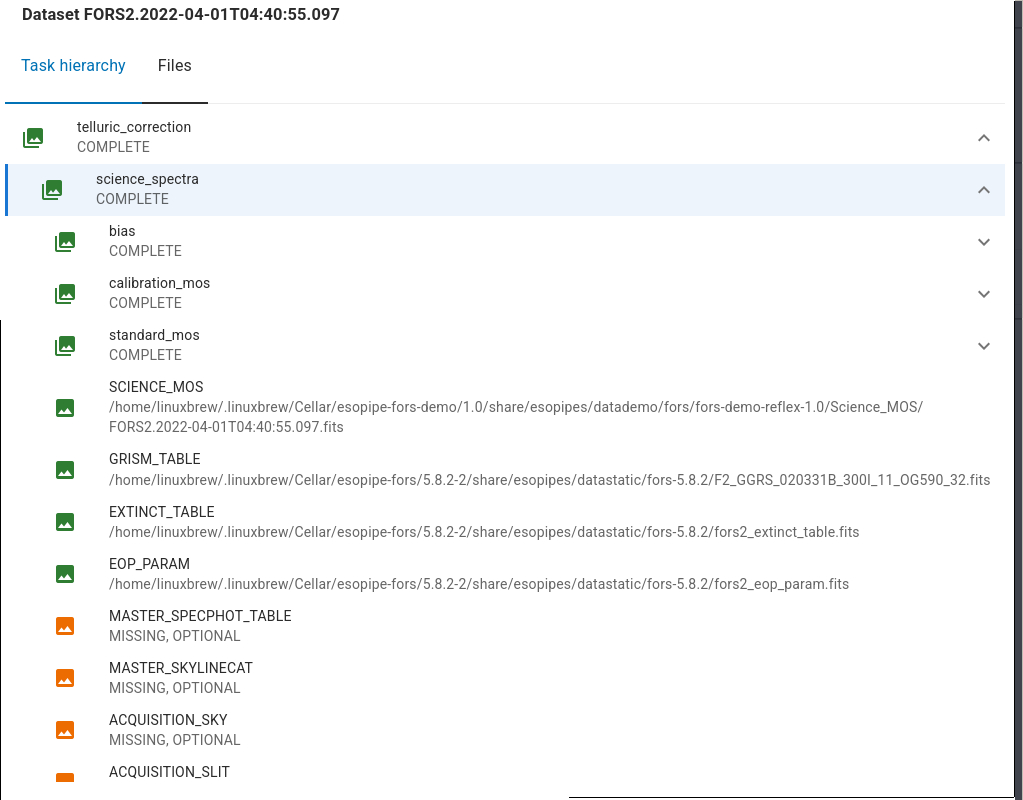
\includegraphics[width=0.9\textwidth]{figures/dataset-tree.jpg}
\caption{The tree-structure of a dataset, illustrating the calibration cascade. Orange and Red symbols show the optional and mandatory calibrations that are missing, respectively}
\label{fig:dataset-tree}
\end{figure}

\end{itemize}
  